% !TEX encoding = UTF-8 Unicode

\documentclass[a4paper,oneside,12pt]{report}

\usepackage{titlesec}
\usepackage[top=2cm, bottom=2cm, left=2cm, right=2cm]{geometry}
\usepackage[T1]{fontenc}
\usepackage[polish]{babel}
\usepackage[utf8]{inputenc}
\linespread{1.3}
\usepackage{textgreek}
\usepackage{lmodern}
\usepackage{amssymb}
\usepackage{amsmath}
\usepackage{fixltx2e}
\usepackage{graphicx}
\usepackage{rotating}

\usepackage{setspace}
\selectlanguage{polish}

\graphicspath{ {images/} }
\makeatletter

\renewcommand{\maketitle}{\begin{titlepage}

	\vspace*{ \stretch{0.1} }
	\begin{center} \LARGE
	\textbf{Uniwersytet Jagielloński w Krakowie} \\
  	Wydział Fizyki, Astronomii i Informatyki Stosowanej
	\end{center}

	\vspace{ \stretch{0.5} }
	\begin{center}
		\large \@author \\
		\vspace{3mm}
		\normalsize Nr albumu: 1124802
	\end{center}

	\vspace{ \stretch{0.1} }
	\begin{center} \Huge
		\textsc {\@title}
	\end{center}

	\vspace{ \stretch{0.1} }
	\begin{center}
	Praca licencjacka\\
	na kierunku Informatyka
	\end{center}

	\vspace{ \stretch{1.5} }
	\begin{flushright}
	\begin{minipage}{8cm}
	\begin{center} \large
	Praca wykonana pod kierunkiem \\
	prof. dr hab. Piotra Białasa \\
	FAIS UJ
	\end{center}
	\end{minipage}
	\end{flushright}
	\vspace{ \stretch{1} }
	\begin{center}
	\@date
	\end{center}
\end{titlepage}
}

\makeatother

\titleformat{\chapter}%
  {\normalfont\bfseries\Huge}{\thechapter.}{10pt}{\Huge}
\titlespacing*{\chapter}{0pt}{0pt}{40pt}
\renewcommand*\contentsname{Spis Treści}

\author{\textbf{Wojciech Ozimek}}
\title{\textbf{Wykorzystanie sztucznych sieci neuronowych do analizy obrazów na przykładzie kostki do gry}}
\date{Kraków 2018}

\begin{document}
\maketitle{}

\tableofcontents
\newpage

% !TEX encoding = UTF-8 Unicode

\chapter{Cel pracy}

Celem pracy jest stworzenie sieci neuronowej rozpoznającej ilość oczek wyrzuconych
na kostce do gry. Sieć powinna rozpoznawać kostki o dowolnym zestawieniu kolorystycznym
ścian oraz oczek i działać na rzeczywistym obrazie przesyłanym z kamery.\\
Dodatkowym aspektem poruszonym w pracy jest porównanie modeli w zależności od
architektury sieci oraz zbiorów danych.


% !TEX encoding = UTF-8 Unicode

\chapter{Wstęp}

Sieci neuronowe składają się ze sztucznych neuronów, które są uproszczonymi modelami ich
biologicznych odpowiedników. Pierwsze prace nad tym zagadnieniem zaczęły sie już w latach 50.
XX wieku.

\section{Sztuczny neuron}

Najprostszym modelem sztucznego neuronu jest tzw. neuron McCullocha-Pittsa, nazywany
również neuronem binarnym. Taki neuron posiada wiele wejść, z których każde ma przypisaną
wagę w postaci liczby rzeczywistej. Suma wartości wejściowych mnożona jest przez odpowiadające
im wagi i podawana jako argument do funkcji aktywacji, wyjaśnionej w późniejszych rozdziałach.
Wartość tej funkcji jest wyjściem neuronu i staje się wejściem innych neuronów,
tak jak ma to miejsce w przypadku biologicznego neuronu \cite{CS231n}.\\
Neurony najczęściej łączone są w struktury nazywane sztucznymi sieciami neuronowymi, ponieważ wykorzystanie
pojedynczego neuronu nie pozwala na rozwiązywanie skomplikowanych zadań.
Przykładowo próba realizacji prostych funkcji logicznych ANR, OR, NOT i XOR okazuje
się możliwa jedynie dla trzech pierwszych podanych funkcji \cite{XORproblem}.
Problem wiąże się z brakiem możliwości uzyskania poprawnych rezultatów dla zbiorów które
nie są liniowo separowalne, czego przykładem jest właśnie funkcja XOR. Tworzenie rozbudowanych
struktur z pojedynczych neuronów znacząco zwiększa możliwości adaptacyjne
dla poszczególnych problemów, niejednokrotnie zaskakując osiąganymi wynikami.

\section{Historia}

Rozpoczęcie prac nad sztucznym neuronem można datować na rok 1943 kiedy
Warren McCulloch i Walter Pitts przedstawili jego model \cite{NNbiology}.
Pierwszymi zastosowaniami sieci neuronowych były operacji bitowe oraz przewidywania kolejnych
wystąpień bitów w ciągu. Mimo licznych prób zastosowania ich do realnych problemów
nie zyskały one popularności. W początkowym okresie rozwoju sieci neuronowych
przyjmowano także wiele błędnych założeń, które wraz z ograniczonymi możliwościami
obliczeniowymi komputerów skutecznie zniechęcały naukowców do prac nad tym zagadnieniem.\\


% !TEX encoding = UTF-8 Unicode

\chapter{Technologie}
Rozwój informatyki i wzrost zainteresowania sieciami neuronowymi spowodowały pojawienie
się wielu, ułatwiających pracę, narzędzi. Wykorzystane w tej pracy technologie
pozwoliły na skupienie się wokół faktycznego problemu i pominięcie wielu technicznych
aspektów.

\section{Język programowania i środowisko}

\paragraph{Python} \mbox{}\\
Kod stworzony na potrzeby tej pracy został napisany w jezyku programowania Python, który
obecnie jest bardzo popularnym narzędziem wykorzystywanym w pracy naukowej.
Podowem jego tego wyboru jest bardzo czytelna i zwięzła składnia,
która w pełni pozwala skupić się na danym problemie. Python jest on także domyślnym
językiem używany w bibliotekach wykorzystywanych do tworzenia modeli sieci neuronowych.

\paragraph{Jupyter Notebook} \mbox{}\\
Do łatwiejszego tworzenia i analizowania modeli sieci neuronowych wykorzystano aplikację
Jupyter Notebook, pozwalającą uruchamiać w przeglądarce pliki, nazywane notebookami,
które składają się z wielu bloków. W blokach może znajdować się wykonywalny kod programu
lub jego fragment, a w pozostałych można prezentować m.in. teksty, wykresy bądź tabele,
co zdecydowanie ułatwia pracę.\\

\section{Biblioteki}

\paragraph{OpenCV} \mbox{}\\
Posiadanie mniejszych niż otrzymywanych bezpośrednio z kamery obrazów bardzo przyśpiesza
naukę sieci neuronowych. Do obróbki obrazów wykorzystano bibliotekę OpenCV.
Najczęsciej wykorzystywana jest w językach C++ oraz Python, pozwalając m.in. na
skalowanie, kadrowanie i obrazanie obrazów.

\paragraph{TensorFlow} \mbox{}\\
TensorFlow jest biblioteką ułatwiającą tworzenie sieci neuronowych. Jej ogromną zaletą
jest implementacja w języku C++ umożliwiająca wykorzystywanie procesorów oraz kart graficznych.
Z uwagi na charakter  wykonywanych obliczeń praca przy użyciu kart graficznych jest
kilkukrotnie szybsza niż na procesorze, co znacząco przyśpiesza proces uczenia.
Biblioteka najlepiej wspiera języki programowania C++ oraz Python.

\paragraph{Keras} \mbox{}\\
Wykorzystywaną w tej pracy biblioteką do tworzenia modeli sieci neuronowych jest Keras,
wykorzystujący bardziej niskopoziomowe biblioteki jak TensorFlow.
Zaletami Kerasa są zarówno przystępny interfejs pozwalający w krótkim czasie stworzyć model
sieci oraz możliwość tworzenia zaawansowanych modeli przy średnim pogorszeniu czasu
uczenia się sieci o 3-4\% w stosunku do bibliotek, na których bazuje.\\
W sytuacji kiedy interfejs oraz dokumentacja do TensorFlow mogą być dla początkującej
osoby niezrozumiałe, jest to świetna alternatywa do wdrożenia się w to zagadnienie.

\paragraph{Numpy} \mbox{}\\
Wykonywanie operacji na dużych zbiorach danych dostarczanych do sieci zostało przyśpieszone
dzięki wykorzystaniu modułu Numpy. Moduł umożliwia wykonywanie zaawansowanych operacji na macierzach
oraz wektorach, wspierający liczne funkcje matematyczne. Jest bardzo rozpowszechniony
i wykorzystywany w wielu, głównie naukowych zastosowaniach. Numpy wprowadza własne
typy danych oraz funkcje niedostępne w standardowej instalacji Pythona.

\paragraph{Matplotlib} \mbox{}\\
Wykresy potrzebne do analizy sieci neuronowych tworzone były przy użyciu narzędzia Matplotlib.
Posiada bardzo duże możliwości pozostając jednocześnie prostym w użyciu co sprawia
jest bardzo popularny. Dodatkowo zawiera moduł pyplot, który w założeniu ma maksymalnie przypominać
interfejs w programie MATLAB.

\paragraph{LaTeX} \mbox{}\\
Oprogramowanie do składu tekstu, nie będące edytorem tekstowy typu WYSIWYG.
LaTeX bazuje na TeX, który jest systemem składu drukarskiego do prezentacji w
formie graficznej. Ogromną zaletą jest możliwość tworzenia w tekście zaawansowanych
wzorów matematycznych. Tekst niniejszej pracy napisany został przy pomocy tego narzędzia.

\section{Technologie wspomagające}
Kilkukrotne przyśpieszenie tworzenia modeli do tej pracy możliwe było dzieki wykorzystaniu
możliwości oferowanych przez szybkie karty graficzne.

\paragraph{NVIDIA CUDA} \mbox{}\\
Technologia obecna w kartach firmy NVIDIA to równoległa architektura obliczeniowa,
pozwalająca na wielokrotne przyśpieszneie obliczeń podczas uczenia się sieci neuronowych.
Dzięki bibliotekom TensorFlow i Keras, które wspierają obliczenia na kartach graficznych,
czas uczenia sieci drastycznie maleje. Podczas tej pracy wykorzystana została
karta NVIDIA TESLA K80 12GB GPU dostępna na Amazon AWS oraz Google Compute Engine.

\paragraph{Amazon AWS EC2} \mbox{}\\
Szybkie karty graficzne wykorzytane w tej pracy były dostępne na plaftormie z
wirtualnymi maszynami, które można dostosować do potrzeb klienta. Wykorzystano maszyny
zoptymalizowane do obliczeń na kartach graficznych i uczenia maszynowego.
Dzięki wykorzystaniu Amazon AWS, czas uczenia sieci zmniejszył się średnio 6-10 krotnie
w stosunku do pracy na komputerze wykorzystującym procesor.


% !TEX encoding = UTF-8 Unicode

\chapter{Słownik pojęć}

\paragraph{Zbiór danych} \mbox{}\\
Zbiór danych lub obrazów to zbiór wszystkich zdjęć kości wykonanych na poczet
pracy z wykorzystaniem kamery. Każde zdjęcie w zbiorze jest przetworzone w celu
zmniejszenia czasu uczenia się sieci oraz potrzebnej pamięci. Zdjęcia były wykonywane
kamerą o rozdzielczości 1600x1200 pikseli. Każde ze zdjeć w zbiorze zostało
poddane procesowi skalowania oraz kadrowania w celu osiągnięcia odpowiedniego
rozmiaru. W celu uzyskania większej liczebności zbioru wszystkie obrazy zostały
dodatkowo poddane operacji obrotu o dany kąt. Każdy ze zbiorów został zduplikowany
i poddany konwersji z trybu RGB na skalę szarości przez usunięcie informacji o barwie
oraz nasyceniu kolorów, pozostawiając jedynie informację o jasności piksela. \\
Po przeprowadzeniu całego procesu, każdy obraz miał wymiary 64x64, zarówno w wersji
kolorowej i czarno białej, co skutkowało rzeczywistymi rozmiarami odpowiednio 64x64x3
oraz 64x64x1.

\paragraph{Zbiór treningowy} \mbox{}\\
Część zbioru danych który wykorzystywany jest w procesie uczenia sieci określany
jest mianem zbioru treningowego lub zbioru uczącego. Jego liczebność to zazwyczaj 60-80\% całego zbioru
danych. Praktycznie we wszystkich zastosowaniach dane w tym zbiorze przed rozpoczęciem
uczenia poddawane są losowej permutacji.

\paragraph{Zbiór testowy} \mbox{}\\
Zbiór testowy lub zbiór walidacyjny służy do oceny zdolności sieci do rozpoznawania
danych. Celem rozdzielenia tego zbioru od danych testowych jest weryfikacja sieci
na danych które wcześniej nie zostały przetworzone przez sieć.

\paragraph{Neuron} \mbox{}\\
Najmniejszy element sieci neuronowej, przyjmuje wiele wejść i jedno wyjście. Może
zawierać także próg (ang. threshold), który może być zmieniony przez funkcje uczącą.
Neuron wyposazony jest także w funkcję aktywacji, odpowiednio modyfikującą jego wyjście.
Każde wyjście neuronu z poprzedniej warstwy połączone jest z wejściami innych neuronów
w warstwie następnej.
\begin{equation}
f(x_{i}) = \sum_{i}w_{i}x_{i} + b \\
\end{equation}

\paragraph{Wagi neuronu} \mbox{}\\
Połączenia w sieci realizowane są między wyjściem poprzedniego neuronu \textit{i}
oraz wejściem następnego neuronu \textit{j}. Każde takie połączenie ma przypisaną
wartość wagi \textit{w\textsubscript{ij}}. Podczas procesu uczenia wagi zmieniają
się, dostosowując sieć neuronową do otrzymywanych danych, co skutkuje
zmniejszeniem wartości błędu.

\paragraph{Bias} \mbox{}\\
Bias to dodatkowa waga wejściowa do neuronu umożliwiająca jego lepsze dopasowanie
do danych treningowych. W sytuacji kiedy wszystkie wagi neuronu mają zerowe
wartości, unikamy problemów podczas procesu wstecznej propagacji.

\paragraph{Warstwa} \mbox{}\\
Sieć neuronowa zorganizowana jest w warstwach. Neurony w danej warstwie nie są
ze sobą w żaden sposób połączone, komunikacja odbywa się tylko między kolejnymi
warstwami. Istnieje wiele rodzajów warstw, a sygnał który przechodzi przez całą
sieć zaczyna się w tzw. warstwie wejściowej oraz kończy w tzw. warstwie wyjściowej.
Istnieją sieci neuronowe (rekurencyjne sieci neuronowe, \textit{(ang. RNN - Recurrent Neural Network)})
w ktorych sygnał może przechodzić przez warstwy kilkukrotnie w trakcie jednej epoki.

\paragraph{Rodzaje warstw} \mbox{}\\
Poniższe rodzaje warstw zostały użyte w modelach przedstawionych w tej pracy.

\subparagraph{Wejściowa}  \mbox{}\\
W pracy, gdzie zbiorami danych są zbiory obrazów, każdy pojedynczy piksel obrazu
odpowiada jednej wartości liczbowej. W związku z tym rozmiar pierwszej warstwy
wejściowej jest identyczny z wymiarami obrazu. Warstwa wejściowa charakteryzuje się
brakiem wejść oraz biasu.

\subparagraph{Wyjściowa}  \mbox{}\\
Rozmiar warstwy wyjściowej odpowiada ilości klas do jakiej wejściowe dane miały
zostać sklasyfikowne. Oczekiwanym wyjściem sieci w pracy była liczba oczek możliwych
do wyrzucenia na kostce, co odpowiada 6 klasom, po jednej na każdą wartość na boku
kostki. Wyjściem wszystkkich przedstawianych w tej pracy sieci był wektor o wymiarach
6x1.

\subparagraph{Konwolucyjna}  \mbox{}\\
Warstwa konwolucyjna służy do przetworzenia danych z poprzedniej warstwy do postaci
filtrów konwolucyjnych o określonych wymiarach w celu znalezienia cech wśród dostarczonych
danych. Więcej informacji na temat sposobu w jaki działa konwolucja, opisane jest w sekcji
\textit{Konwolucja} oraz \textit{Konwolucyjna sieć neuronowa}.

\subparagraph{Aktywacyjna}  \mbox{}\\
Jest to wydzielenie funkcji aktywacji do osobnej warstwy, które jest realizowane
w niektórych bibliotekach. Celem takiego zabiegu jest możliwości podglądu danych
na wyjściu neuronu, tuż przed zaaplikowaniem funkcji aktywacji.

\subparagraph{W pełni połączona}  \mbox{}\\
Sieć neuronowa składa się z w pełni połączonych warstw \textit{(ang. Fully Connected, Dense)}.
W konwolucyjnych sieciach neuronowych warstwy te występują po warstwach konwolucyjnych
i służą do powiązania nieliniowych kombinacji które miały zostały wygenerowane przez
warstwy konwolucyjne oraz ich klasyfikowania. Dodatkowo nie wymagają dużych nakładów
obliczeniowych i są proste do zaaplikowania. Swoją nazwę biorą od sposobu w jaki
realizowane sa połączenia między warstwami. Neurony z poprzedniej warstwy łączą się ze
wszystkimi neuronami następnej warstwy.

\subparagraph{Flatten}  \mbox{}\\
Warstwa spłaszczająca \textit{(ang. Flatten)} stosowana jest w celu połączenia warstw
konwolucyjnych lub aktywacji wraz z warstwami w pełni połączonymi. Realizowane jest
to poprzez przekształcenie warstwy wejściowej do jednowymiarowego wektora który następnie
służy za wejście do kolejnych warstw.

\subparagraph{Odrzucająca}  \mbox{}\\
Warstwa odrzucająca \textit{(ang. Dropout)} zapobiega przetrenowaniu \textit{(ang. Overfitting)}
sieci. Proces ten polega na nie braniu pod uwagę wyjść pewnych neuronów, zarówno
w przypadku przechodzenia w przeód oraz w tył. Stosuje się ją po warstwach w pełni
połączonych, w celu zapobiegania rozległym zależnościom między neuronami. W warstwie
tej określone jest prawdopodobieństwo \textit{p} z jakim neuron zostanie zachowany
w warstwie oraz \textit{p - 1} z jakim zostanie odrzucony.


\subparagraph{MaxPooling}  \mbox{}\\
Warstwa tzw MaxPoolingu wykorzystywana jest do zmniejszenia rozmiaru pamięci oraz
ilości obliczeń wymaganych przez sieć neuronową, jak również może zapobiegać przetrenowaniu.
Operacja zmniejszenia polega na wybraniu jednego piksela z danego obszaru, w przypadku
MaxPoolingu, takiego o największej wartości i przekazaniu go dalej. Obszar z jakiego
wybieramy dany piksel jest zależy od danej warstwy, ale najczęściej jest to kwadrat
o wymiarach 2x2 co oznacza znaczące ograniczenie zużycia pamięci i koniecznych obliczeń.
MaxPooling jest krytykowany ponieważ nie zachowuje informacji o połozeniu piksela
przekazanego na wyjście warstwy co może objawiać się błednymi interpretacjami
podczas testowania sieci.



\paragraph{Funkcja aktywacji} \mbox{}\\
Przy pomocy funkcji aktywacji obliczana jest wartość wyjściowa neuronów w sieci
neuronowej. Argumentem dostarczanym do funkcji aktywacji jest suma wejść neuronu
pomnożonych przez przypisane im wartości wag. Zależnie od konkretnego rodzaju funkcji
aktywacji, neuron po przekroczeniu danego progu wysyła sygnał wyjściowy, odbierany
przez neurony znajdujące się w następnej warstwie.
\begin{equation}
f\Big(\sum_{i}w_{i}x_{i} + b\Big) \\
\end{equation}

\paragraph{Rodzaje funkcji aktywacji} \mbox{}\\
Przedstawione poniżej funkcje aktywacji zostały użyte w modelach zaprezentowanych
w tej pracy.

\subparagraph{Liniowa} \mbox{}\\
Funkcja ta jest praktycznie nie wykorzystywana w sieciach neuronowych. Połączenie
wielu warstw których neurony posiadają liniową funkcję aktywacji można przedstawić
za pomocą jednej warstwy,  ponieważ złożenie wielu funkcji liniowych również będzie
funkcją liniową. Nieliniowość funkcji pozwala na klasyfikacje danych przechodzących
przez sieć.
\begin{equation}
f(x) = x
\end{equation}


\subparagraph{Sigmoid} \mbox{}\\
Największym problemem funkcji sigmoidalnej jest duże ryzyko zaniknięcia gradientu,
co może prowadzić do problemu tzw umierającego neuronu. Zjawisko to ma miejsce
gdy dla danej funkcji aktywacji, gradient staję się bardzo mały. Jest równoznaczne
z zaprzestaniem procesu uczenia, ponieważ gradient zera również wynosi zero.
W przypadku tej funkcji gradient może zanikać obustronnie.
\begin{equation}
f(x) = \sigma(x) = \frac{1}{1 + e^{-x}} \\
\end{equation}

\subparagraph{Tanh} \mbox{}\\
\begin{equation}
f(x) = tanh(x) = \frac{(e^x - e^{-x})}{(e^x + e^{-x})} \\
\end{equation}

\subparagraph{ReLU} \mbox{}\\
ReLU \textit{(and. Rectified linear unit)} jest najpopularniejszą funkcją aktywacji
wykorzystywaną w sieciach neuronowych. Zasługą tego jest szybki czas uczenia sieci
bez znaczącego kosztu w postaci generalizacji dokładności. Problem z zanikającym
gradientem jest mniejszy niż w przypadku funkcji sigmoidalnej, ponieważ występuje
on tylko z jednej strony.
\begin{equation}
f(x) = max(0, x) =
\begin{cases}
 x & \text{if } x \geqslant 0 \\
 0 & \text{if } x < 0 \\
\end{cases}
\end{equation}

\subparagraph{LeakyReLU} \mbox{}\\
LeakyReLU jest ulepszeniem ReLU dzięki zastosowaniu niewielkiego gradientu w sytuacji
dla której ReLU jest nieaktywne. Zmiana ta pozwala na uniknięcie problemu tzw
umierającego neuronu.
\begin{equation}
f(x) =
\begin{cases}
 x & \text{if } x \geqslant 0 \\
 0.01x & \text{if } x < 0 \\
\end{cases}
\end{equation}

\paragraph{Funkcja kosztu} \mbox{}\\
Funkcja kosztu lub funkcja błędu jest niezbędna do prawidłowego przeprowadzenia
procesu uczenia. Daje ona informacje o różnicy między obecnym staniem sieci o
optymalnym rozwiązaniem. Algorytm uczenia sieci analizuje wartość funkcji kosztu
w kolejnych krokach w celu zminimalizowania jej.

\paragraph{Propagacja wsteczna} \mbox{}\\
Propagacja wsteczna lub wsteczna propagacja błędów \textit{(ang. Backpropagation)}
jest jednym z najskuteczniejszych algorytmów uczenia sieci neuronowych. Polega
na minimalizacji funkcji kosztu korzystając z metody najszybszego spadku lub
bardziej zoptymalizowanych sposobów, o których napisane jest w sekcji \textit{Optymalizator}.
Swoją nazwę zawdzięcza sposobowi w jaki propagowane są te błędy, od warstwy
wyjściowej do wejściowej.

\paragraph{Optymalizator} \mbox{}\\
Inne określenie algorytmu optymalizacyjnego wykorzystywanego do obliczania wag neuronów
i biasu sieci neuronowej. Posiada kluczowe znaczenie podczas procesu uczenia sieci
zarówno w kwestii czasu oraz skuteczności. Z tego powodu jest to jeden z kluczowych
obszarów obecnych badań i rozwoju sieci neuronowych.

\subparagraph{Metoda gradientu prostego} \mbox{}\\
Metoda gradientu prostego \textit{(ang. Gradient Descent)} jest podstawowym algorytmem
służacym do uaktualniania wartości wag oraz biasu podczas uczenia sieci. Wadą tej
metody jest przeprowadzanie jednorazowej aktualizacji po wyliczeniu gradientu dla
całego zestawu danych. Jest to bardzo wolne, w niektórych przypadkach może powodować
problem z ilością zajmowanego miejsca w pamięci a przede wszystkim może prowadzić
do pozostania w jednym z lokalnych minimów funkcji.
\begin{equation}
\theta = \theta - \eta * \nabla J(\theta)
\end{equation}

\subparagraph{Stochastic Gradient Descent} \mbox{}\\
\textit{(nazwa w języku angielskim z powodu braku znalezienia polskiego odpowiednika)}
Stochastic Gradient Descent \textit{(skrót. GDA)} jest rozwinięciem metody gradientu
prostego, bardzo często wykorzystywana w praktyce. Ulepszenie polega na obliczaniu
gradientu dla jednego lub niewielkiej ilości przykładów treningowych. Najczęsciej
korzysta się z więcej niż jednego przykładu co zapewnia lepszą stabilność oraz
wykorzystuje zrównoleglanie obliczeń. SGD zapewnia to większą rozbieżność niż metoda
gradiento prostego, co umożliwia znajdowanie nowych lokalnych minimów ale wiąże się
z koniecznością zastosowania mniejszego stopnia uczenia.
\begin{equation}
\theta = \theta - \eta * \nabla J(\theta; x_i; y_i)
\end{equation}

\subparagraph{RMSprop} \mbox{}\\
RMSprop umożliwia obliczanie gradientu dla każdego parametru z osobna i zapobiega
zmniejszaniu się stopnia uczenia. Algorytm dostosowuje stopień uczenia dla każdej wagi
bazując na wielkości jej gradientu.

\subparagraph{Adam} \mbox{}\\
Adam to skrót od angielskiej nazwy \textit{Adaptive Moment Estimation} i jest rozwinięciem
metody Stochastic Gradient Descent. Metoda ta pozwala na obliczanie z osobna gradientu dla
każdego parametru oraz każdej zmiany momentum. Zapobiega dodatkowo zmniejszającemu się
stopniowi uczenia, a co najważniejsze jest bardzo szybka i pozwala na sprawne uczenie
się sieci. W tej metodzie obliczamy dwa momenty \textit{m} oraz \textit{v}.
\begin{equation}
\begin{align*}
\hat{m_t} = \frac{m_t} {1 - \beta^t_1}, \\
\hat{v_t} = \frac{v_t} {1 - \beta^t_2}, \\
\end{align*}
\end{equation}
Powyżej obliczone momenty podstawiamy do wzoru
\begin{equation}
\theta_{t+1} = \theta_t - \frac {\eta} {\sqrt{\hat{v_t}} + \epsilon} \hat{m_t}
\end{equation}
gdzie najczęściej \textbeta \textsuperscript{t}\textsubscript{1} = 0.9 oraz
\textbeta \textsuperscript{t}\textsubscript{2} = 0.99 a \straightepsilon = 10^{-8}\\

\paragraph{Sieć neuronowa} \mbox{}\\

\paragraph{Konwolucja} \mbox{}\\

\paragraph{Filtr konwolucyjny} \mbox{}\\

\paragraph{Konwolucyjna sieć neuronowa} \mbox{}\\

\paragraph{Paradygmaty uczenia} \mbox{}\\

\paragraph{Epoka} \mbox{}\\
Proces uczenia sieci podzielony jest na epoki. Każda epoka odpowiada przejściu
wszystkich elementów z treningowego zbioru danych przez sieć. Ilość epok podczas
których sieć będzie sie uczyć ustala się na co najmniej kilkanaście. W przypadku
większych zbiorów danych lub większych modeli sieci zwiększamy ilość epok. \\
Często spotykaną praktyką w wielu pracach naukowych jest przedstawianie wyników
dla sieci po 100 epokach uczenia się.

\paragraph{Uczenie} \mbox{}\\
Proces uczenia bądź treningu sieci służy zmianie wartości wag, najczęściej zainicjowanych
pseudolosowymi wartościami oraz biasu. Uczenie się sieci neuronowej jest bardzo
kosztowne obliczeniowo, co wręcz uniemożliwiało trenowanie modeli w przeszłości,
a obecnie jest jednym z powodów dużego technologicznego przeskoku w produkcji kart
graficznych. Operacje dodawania i mnożenia wektór i macierzy wykonywane są setki
milionów razy, które mogą być przyśpieszone dzięki możliwościom zrównoleglania obliczeń. \\

\paragraph{Testowanie} \mbox{}\\
Model sieci neuronowej może zostać poddany ocenie, dzięki której można określić w jakim stopniu
nauczyła się sieci. W przypadku wytrenowanych modeli istotne jest aby zbiór służący do
testowania nie był wcześniej użyty do treningu sieci. Nauczony model powinien być w stanie
rozpoznawać nowe, nieużyte podczas procesu uczenia dane i poprawnie je klasyfikować.

\paragraph{Predykcja} \mbox{}\\
Wartości zwrócone przez sieć po umieszczeniu w niej określonych danych są określane
mianem predykcji. Pozwala to na wykorzystanie nauczonego modelu w praktycznym
zastosowaniu. \\ \\ \\

Tematy do uwzględnienia:
minibatch,
nesterov,
momentum,
softmax,
learning rate,
categorical crossentropy,
Liczebność zbioru (konkretne uzasadnienie konieczności duzej liczby danych),
one-hot encoding,
hyperparameters: ilosc filtrow, rozmiar filtrow, rozmiar maxpoolingu


% !TEX encoding = UTF-8 Unicode

\chapter{Tworzenie zbiorów danych}
Aby sieć neuronowa mogła rozpoznawać obrazy, konieczne jest stworzenie danych
do jej nauki i testowania. Priorytetem przy ich tworzeniu było
umożliwienie rozwoju różnych modeli sieci neuronowych bez konieczności każdorazowej
zmiany w zbiorach lub dopasowywania ich do konkretnej sieci.\\
\textbf{Wszystkie zbiory dostępne są pod linkami w części Dodatek A [\ref{dodatekA}.] }

\section{Uzyskiwanie zbiorów ze zdjęć}
Ilość zdjęć wykonanych ręcznie z wykorzystaniem kamery była zbyt mała by sieć bezpośrednio
z nich korzystała. Oprócz tego rozmiar zdjęć 1600x1200 był na tyle duży, że bardzo wydłużyłby
proces uczenia sieci.\\
Rozwiązaniem obu problemów było zwiększenie ilości zdjęć przy jednoczesnym zmniejszeniu
ich rozmiarów. Do wszystkich obrazów wykorzystywanych w tej pracy, zastosowano następujące
kroki:
\begin{itemize}
\item Skalowanie obrazów
\item Przekształcanie \textit{(ang. warping)} na kilka różnych sposobów, by uzyskać lekko zdeformowane kostki
\item Rotacja o określony kąt by umożliwić rozpoznawanie kości niezależnie od jej obrotu
\item Kadrowanie obrazu do pożądanej wielkości
\end{itemize}
Wszystkie zbiory wykorzystane w tej pracy były podzielone na części treningową i testową
w stosunku 4:1, niezależnie od ich liczebności.

\section{Zbiór obrazów kwadratowych}
Pierwszy stworzony zbiór składał się z obrazów kwadratowych. Było to podyktowane
faktem, że praktycznie wszystkie przykłady użycia sieci neuronowych do rozpoznawania
obrazów korzystały z kwadratowych zdjęć.\\
Najważniejszym założeniem przy tworzeniu zbioru było uzyskanie zdjęć kości położonej
na środku obrazu z kamery, na obszarze kwadratu o boku długości około 3 krotnie większej
niż długość ściany samej kości. Pozwalało to uzyskać niewielkie rozmiary obrazów 64x64 piksele,
gdzie kość stanowiła około 14\%, a jedno oczko 0,2\% powierzchni.\\
Kolejną kwestią było przystosowanie sieci do rozpoznawania kości o różnych kolorach ścian,
oczek i samego tła. Zdjęcia podzielono na zestawy, z których każdy miał ustaloną
barwę tła, kości oraz oczek. Każda ścianka sfotografowana była od 3 do 30 razy, dając
liczebność każdego z zestawów miedzy 18 a 180 zdjęć. Niektóre zdjęcia poddawane były
działaniu ostrego, punktowego światła w celu wygenerowania trudniejszych do rozpoznania obrazów.
Zestawienia kolorystyczne wypisane są w tabeli poniżej \ref{tab:zestawienie1}.

\begin{table}[h!]
\centering
\begin{tabular}{rcl|cc}
\multicolumn{3}{c}{Kolor} & \multicolumn{2}{c}{Ilość zdjęć} \\ \hline
kości & oczek & tła & ściany & kostki \\ \hline
biały & czarny & czerwony & 30 & 180 \\
biały & czarny & granatowy & 3 & 18 \\
biały & czarny & czarny & 8 & 48 \\
beżowy & czarny & czerwony & 3 & 18 \\
czarny & biały & czarny & 10 & 60 \\
czarny & biały & czerwony & 10 & 60 \\
czerwony & biały & czerwony & 5 & 30 \\
czerwony & czarny & czerwony & 3 & 18 \\
granatowy & złoty & biały & 4 & 24 \\
granatowy & złoty & niebieski & 6 & 36 \\
zielony & biały & zielony & 8 & 48 \\
zielony & biały & biały & 5 & 30 \\
różowoczerwony & czarny & biały & 5 & 30 \\ \hline
\multicolumn{3}{c}{\textit{Łączna ilość zdjęć:}} & \textit{100} & \textit{600}
\end{tabular}
\vspace{0.2cm}
\caption{Zestawienie kolorystyczne obrazów 1}
\label{tab:zestawienie1}
\end{table}
Po wykonaniu zdjęć każde z nich zostało poddane obróbce w celu zmniejszenia i uzyskania licznych,
zróżnicowanych zbiorów. W przypadku zbioru kwadratowego wszystkie zdjęcia zostały przeskalowane
do 18,66\% początkowego rozmiaru (stosunek 5,36:1). Następnie poddano je 6 przekształceniom,
które zaprezentowano poniżej (zob. rys. \ref{fig:warping6}):
\begin{figure}[h!]
\centering
\includegraphics[scale=0.8]{warping6}
\caption{Przekształcenia obrazów. Oryginalny obraz znajduje się po lewej.}
\label{fig:warping6}
\end{figure}\\
Kolejnym krokiem był obrót o kąt
15\textsuperscript{o} lub 30\textsuperscript{o}, zależnie czy dany zbiór wykorzystywany był w mniej
lub bardziej rozbudowanych sieciach. Ostatnią operacją było kadrowanie zdjęć do rozmiaru 64x64 piksele.\\
Ostatecznie uzyskano 84 lub 168 zdjęć o rozmiarze 64x64 z każdego
z początkowych obrazów o rozmiarze 1600x1200 pikseli. Pełne zbiory liczyły 50400 i 100800
obrazów, jednakowo w wersjach kolorowych RGB oraz w odcieniach skali szarości.
Wybrane zdjęcia ze zbioru znajdują się (zob. rys. \ref{fig:squares}) poniżej: \newpage

\begin{figure}[h!]
\centering
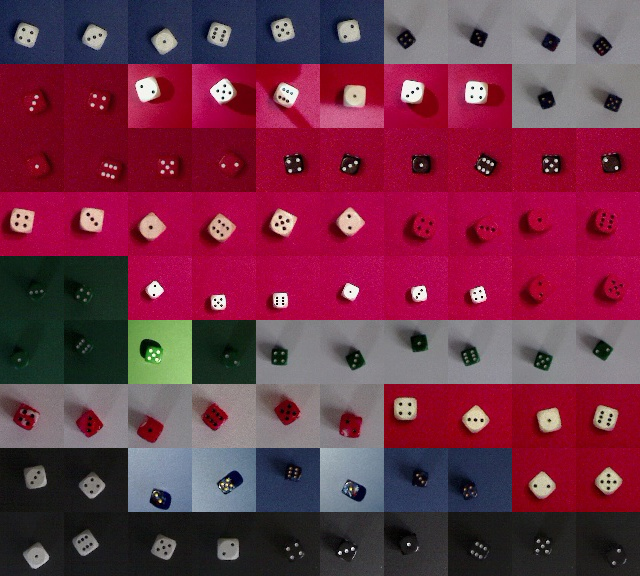
\includegraphics[scale=0.35]{images/kolaz}
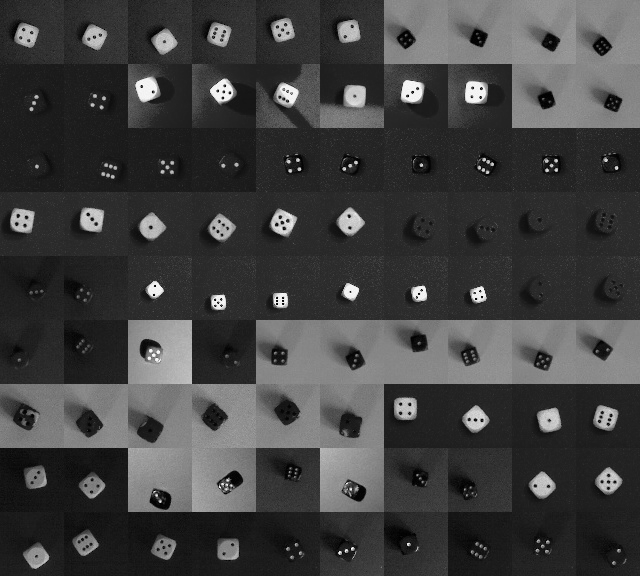
\includegraphics[scale=0.35]{images/kolaz_grayscale}
\caption{Obrazy o rozdzielczościach 64x64}
\label{fig:squares}
\end{figure}

\section{Zbiór obrazów prostokątnych}
Po wytrenowaniu kilku sieci na zbiorach kwadratowych, zdecydowano się na wykorzystanie
większych obrazów, które zachowują kształt prostokątny i stosunek szerokości do wysokości
identyczny z obrazem otrzymywanym z kamery. Miało to ułatwić detekcję kości na obrazie,
ponieważ obszar 64x64 pikseli był na tyle mały, że ciężko byłoby w niego trafić podczas
rzutu kostką.\\
Bardzo istotną rzeczą w tym zbiorze był fakt, że pomimo większego rozmiaru zdjęć, stosunek
rozmiaru kości do całego zdjęcia był zdecydowanie mniejszy. W zdjęciach kwadratowych kostka
zajmowała 14\%, natomiast w prostokątnych jedynie 2\% powierzchni obrazu, a dodatkowo pojedyncze
oczko to tylko 0,08\% powierzchni.
Dla zwiększenia trudności kości były rozmieszczane w bardziej zróżnicowany sposób, nie skupiały
się jedynie wokół środka obrazu. Do wykonanych na potrzeby poprzedniego zbioru zdjęć dodano
nowe i tak utworzono kilkanaście zestawień kolorystycznych, przedstawionych w poniższej tabeli \ref{tab:zestawienie2} \newpage

\begin{table}[h!]
\centering
\begin{tabular}{rcl|cc}
\multicolumn{3}{c}{Kolor} & \multicolumn{2}{c}{Ilość zdjęć} \\ \hline
kości & oczek & tła & ściany & kostki \\ \hline
biały & czarny & czerwony & 30 & 180 \\
biały & czarny & granatowy & 3 & 18 \\
biały & czarny & czarny & 8 & 48 \\
beżowy & czarny & czerwony & 3 & 18 \\
czarny & biały & czarny & 10 & 60 \\
czarny & biały & czerwony & 10 & 60 \\
czerwony & biały & czerwony & 5 & 30 \\
czerwony & czarny & czerwony & 3 & 18 \\
granatowy & złoty & biały & 4 & 24 \\
granatowy & złoty & niebieski & 6 & 36 \\
zielony & biały & zielony & 8 & 48 \\
zielony & biały & biały & 5 & 30 \\
różowoczerwony & czarny & biały & 5 & 30 \\ \hline
biały & czarny & zielony & 6 & 36 \\
czerwony & biały & zielony & 6 & 36 \\
czerwony & czarny & różowy & 7 & 42 \\
czarny & biały & szary & 6 & 36 \\
czarny & biały & niebieski & 6 & 36 \\
beżowy & czarny & szary & 6 & 36 \\
beżowy & czarny & niebieski & 6 & 36 \\
granatowy & złoty & biały & 8 & 48 \\
zielony & biały & żółty & 7 & 42 \\
różowoczerwony & czarny & pomarańczowy & 6 & 36 \\ \hline
\multicolumn{3}{c}{\textit{Łączna ilość zdjęć:}} & \textit{164} & \textit{984}
\end{tabular}
\vspace{0.2cm}
\caption{Zestawienie kolorystyczne obrazów 2}
\label{tab:zestawienie2}
\end{table}
Tak jak poprzednio, zdjęcia zostały poddane obróbce. Początkowo wszystkie zostały
przeskalowane do 16,5\% początkowego rozmiaru (stosunek 6:1). Następnie poddano je 4,
analogicznym jak poprzednio przekształceniom, które pokazano poniżej (zob. rys. \ref{fig:warping4}):
\begin{figure}[h!]
\centering
\includegraphics[scale=0.8]{warping4}
\caption{Przekształcenia obrazów. Oryginalny obraz znajduje się po lewej.}
\label{fig:warping4}
\end{figure}\\
Dokonano również rotacji o kąt 30\textsuperscript{o} i kadrowanie zdjęć do rozmiaru 106x79 pikseli.\\
Uzyskano w ten sposób 60 zdjęć o rozmiarze 106x79 z każdego początkowego zdjęcia.
Obrazy zastosowane w sieciach występowały jedynie w odcieniach skali szarości.
Całkowita ilość obrazów w pełnym zbiorze danych wynosiła 59040, co przełożyło się
na 47232 obrazów treningowych i 11808 testowych. Przykładowe zdjęcia ze zbioru znajdują
się na (zob. rys. \ref{fig:rects}) poniżej:

\begin{figure}[h!]
\centering
\includegraphics[scale=0.5]{dices_106x79}
\caption{Obrazy o rozdzielczościach 106x79}
\label{fig:rects}
\end{figure}


% !TEX encoding = UTF-8 Unicode

\chapter{Sieć rozpoznająca ilość oczek}
W momencie zrobienia zbioru danych składających się z kwadratowych obrazów, przystąpiono
do próby stworzenia i nauczenia modelu sieci neuronowej rozpoznającego ilość oczek
wyrzuconych na kostce do gry.\\
\textbf{Odnośniki do wszystkich modeli dostępne są pod linkami w części Dodatek B [\ref{dodatekB}] }

\section{Hipotezy}
Przed przystąpieniem do tworzenia zbioru danych pojawiła się spora ilość wątpliwości.
Większość z nich dotyczyła kwestii możliwości jakiegokolwiek rozpoznania ilości oczek
przez sieć. Obawy te wiązały się z faktem, że dla przykładu
w zbiorze MNIST, położenie cyfr na obrazie było stałe. W przypadku kiedy na obrazach
kolor biały był obszarem w kształcie przypominającym pionową kreskę, z dużym
prawdopodobieństwem można było założyć że jest to cyfra 1 lub 7, a analogiczna
sytuacja zachodziła dla innych cyfr. W rozpoznawaniu oczek na kostce, zarówno sama
kostka mogła być umieszczona w różnych miejscach na obszarze całego obrazu, jak również
dopuszczalny był jej obrót o dowolny kąt.\\
Następną kwestią był niewielki rozmiar oczka w stosunku do powierzchnii całego ekranu.
W przypadku zbioru MNIST średnio około 12-15\% obrazu stanowiła barwa biała, która
decydowała o wartości zwróconej przez sieć. W przypadku kwadratowych zdjęć z kostkami,
rozmiar jednego oczka to jedynie 0,21\% powierzchnii rozmiaru, a dla obrazów prostokątnych
wartość ta maleje do około 0,08\%. Oznaczało to, że nawet niewielki szum lub
zniekształcenia mogą utrudnić prawidłowe rozpoznanie kości.

\section{Pierwsze eksperymenty z sieciami neuronowymi}
\paragraph{Pierwszy model} \mbox{}\\
Pierwsza próba stworzenia sieci, mając na uwadze wyżej wspomniane wątpliwości, miała
na celu wytrenowanie możliwie prostego zbioru obrazów. W tym celu wykorzystano jedynie
najbardziej liczny zbiór obrazów z czerwonym tłem, białą kością o czarnymi oczkami. Dla
zwiększenia liczby zdjęć w zbiorze, zmniejszono kąt obrotu każdego z nich do
5\textsuperscript{o}, uzyskując 60480 zdjęć ze 120 oryginalnych.\\
Architektura tej sieci, była dobierana bez większego wdrażania się w szczegóły i
bazowała na modelach sieci udostępnionych na stronach Keras oraz TensorFlow,
wykorzystywanych do analizy zbiorów MNIST oraz CIFAR10. Za optymalizator został wybrany
Adam, a sam trening został ustalony na 25 epok w pierwszej turze oraz 10 epok w drugiej
turze. Nigdzie wcześniej nie zauważono tego typu praktyki, aby rozdzielać epoki uczenia.
Zrobiono to dlatego, aby umożliwić wcześniejsze zakończenie całego procesu w sytuacji
gdyby nie zauważono żadnych postępów. Dodatkowo pozwoliło to na zachowanie modelu
po 25 epokach, który mimo że mógłby nie osiągać dobrych rezultatów, pozwoliłby
na wyciągnięcie wniosków lub dalszą naukę. Model sieci prezentował się następująco:\\
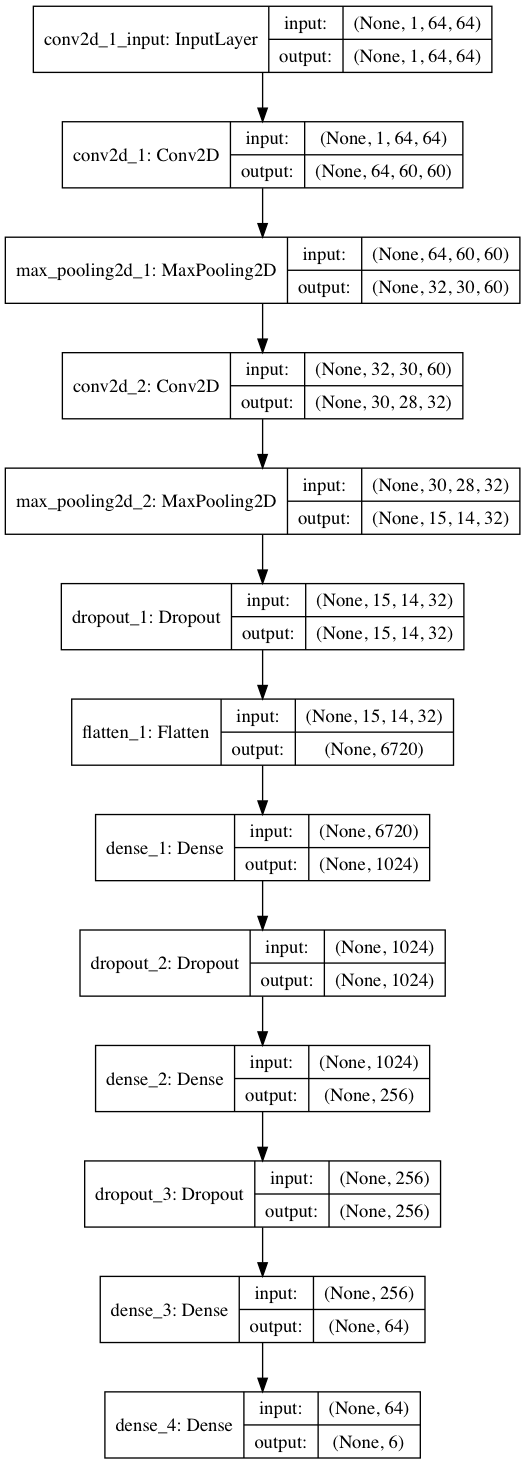
\includegraphics[scale=0.35]{pierwszy_plot}
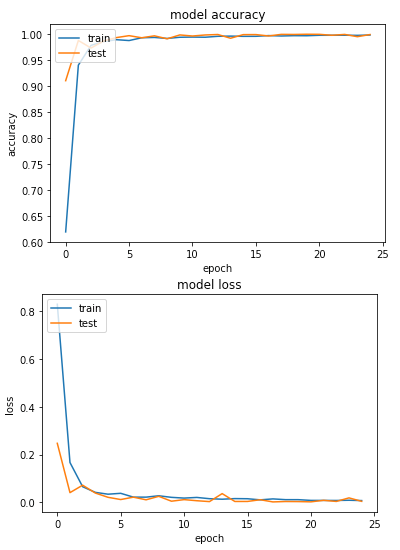
\includegraphics[scale=0.55]{pierwszy_accloss.png}

Rezulataty osiągnięte przez ten model były zdumiewające. Po pierwszej epoce
sieć uzyskała 61,98\% skuteczności ostatecznie osiągając wynik 99,88\% po 25 epokach.
Kolejne 10 epok praktycznie nie poprawiło już tego rezultatu.\\
Po analizie tego dokonania, okazało się że tak duża ilość zdjęć otrzymanych
z każdego ze zdjęć początkowych stworzyła zbiór w którym wiele zdjęć praktycznie się
powtarzało. Sieć nie miała żadnych problemów podczas testowania na zbiorze
do którego w teorii nie miała dostępu podczas treningu. Ten fakt spowodował konieczność
trenowania sieci na zbiorach zróżnicowanych pod kątem doboru różnych kolorów oraz
ilości zdjęć otrzymanych z jednego poczatkowego zdjęcia.

\paragraph{Model ze zróżnicowanymi zdjęciami} \mbox{}\\
Po stworzeniu modelu który wykazał, że zadanie stworzenia dobrze działającej sieci dla
tego problemu jest wykonalne, zabrano się do kolejnego etapu prac. W tym celu
wykorzystano zbiór złożony z 13 różnych zestawów kolorystycznych kości, oczek oraz tła,
liczący po 80640 i 20160 zdjęć na części treningową i testową.\\
W tym modelu wykorzystano architekturę nieznacznie zmienioną w stosunku pierwszego modelu.\\
Sieć uczona była przez 25, a następnie przez 10 epok.
Po pierwszych 25 epokach uzyskano dokladność 55,64\% co potwierdziło przypuszczenie
z przedniej sieci o możliwości pokrycia się zdjęć w zbiorach treningowym i testowym.
Kolejne 10 epok poprawiło wynik sieci do 65,30\%, pozwalając przy okazji zaobserwować
istotny fakt. W pierwszej sesji 25 epok, dokładność sieci przez ostatnie
5 epok oscylowała w okolicach 52\%. W drugiej sesji, niemalże od razu wartość
podniosła się do 56\%. Prawdopodobnie miało to związek ze sposobem w jaki dostarczane
są dane do modelu. Dane były ustalane losowo, ale dla każdej epoki w jednej sesji,
układ ten się nie zmieniał. Istniała szansa, że kiedy w następnej sesji zdjęcia
były przetwarzane w innej kolejności, umożliwiło to lepsze dopasowanie sieci i efekt
skoku jej dokładności.\\
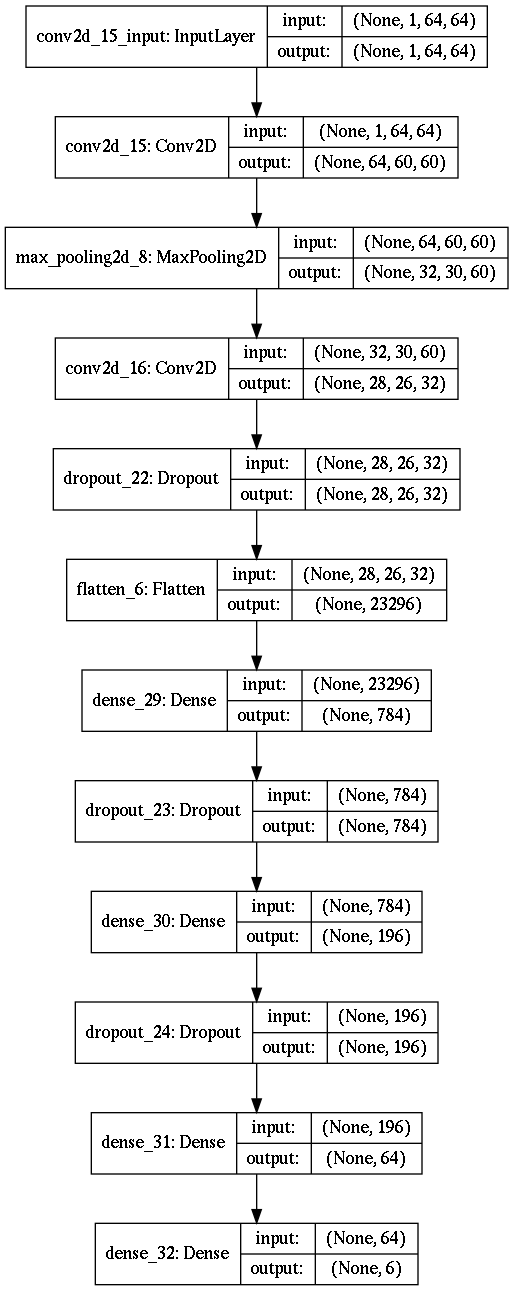
\includegraphics[scale=0.4]{modeladam_plot}
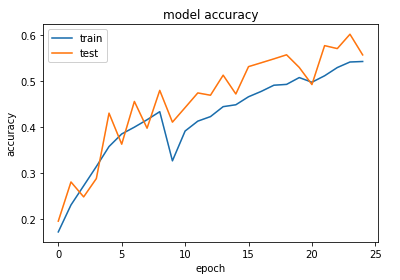
\includegraphics[scale=0.55]{adam_acc}

\paragraph{Model z wybranymi zdjęciami} \mbox{}\\
Znacząca różnica w dokładności między modelem z jednolitymi oraz zróżnicowanymi zdjęciami
doprowadziła do stworzenia sieci uczonej na zbiorze różnorodnych obrazów, ale
dobranymi tak, aby kontrast między tłem, a kością był wyraźny. Architektura sieci
jest identyczna jak w powyższych przykładach, jedyną różnicą jest przetwarzanie
wyselekcjonowanych obrazów. Zastosowanie 25 epok wystarczyło aby uzyskać dokładność
na poziomie 89,23\% co jest rezultatem zdecydowanie lepszym niż uzyskane wcześniej 55,64\%.\\
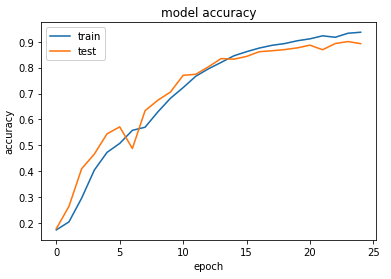
\includegraphics[scale=0.55]{adam_wybrane_acc}
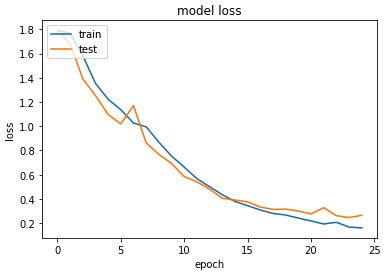
\includegraphics[scale=0.55]{adam_wybrane_loss}

\section{Analiza różnych optymalizatorów}
Jeżeli sama różnica w doborze konkretnych obrazów potrafi w tak dużym stopniu zmienić wyniki
otrzymane przez sieć, podjęto próbę przetestowania kilku z dostępnych w bibliotece Keras
optymalizatorów dla identycznych sieci oraz zbiorów danych. W tym celu postanowiono użyć
optymalizatorów RMSprop oraz SGD.\\
Oba modele z optymalizatorami RMSprop oraz SGD, zostały podobnie jak wcześniej opisany model
z optymalizatorem Adam poddane uczeniu przez 25 epok różnorodnych zbiorów obrazów. Wynik RMSprop
był zdecydowanie najlepszy i wyniósł 84,34\% skuteczności. Najgorszy rezultat w zestawieniu
uzyskał amodel korzystający z SGD, zdobywając jedynie 36,92\% poprawności. Pośrednim okazał
się Adam, który jak opisane wyżej, uzyskał 55,64\% po sesji uczenia przez 25 epok.\\
Wyniki te dowiodły, że optymalizator jest kluczowym parametrem \textit{(ang. hyperparameter)}
dla odpowiednio skutecznego uczenia. Uzyskany wynik dla RMSprop jest sporym zaskoczeniem,
ponieważ w licznych tekstach naukowych to Adam uznawany jest za jeden z najlepszych
optymalizatorów, ciesząc się ogromną popularnością. Również z tego powodu, pomimo
gorszego niż RMSprop wyniku, Adam będzie wykorzystywany w następnych modelach.\\
\textbf{Adam:}\\
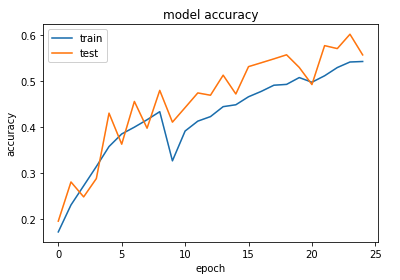
\includegraphics[scale=0.55]{adam_acc}
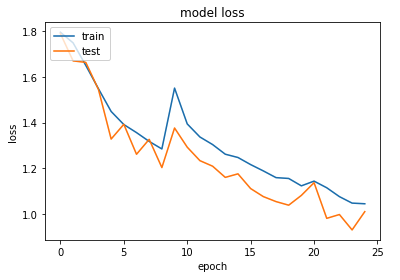
\includegraphics[scale=0.55]{adam_loss}\\
\textbf{RMSprop:}\\
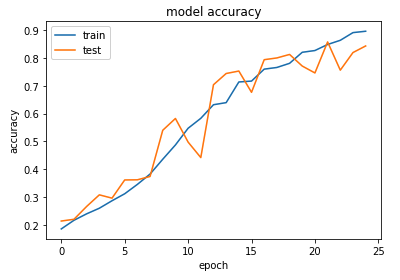
\includegraphics[scale=0.55]{rmsprop_acc}
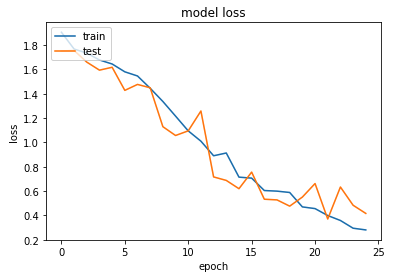
\includegraphics[scale=0.55]{rmsprop_loss}\\
\textbf{SGD:}\\
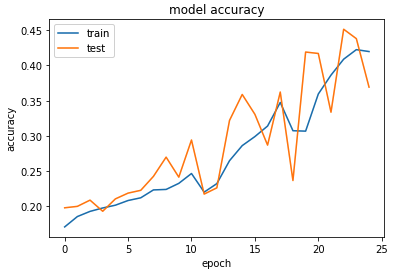
\includegraphics[scale=0.55]{sgd_acc}
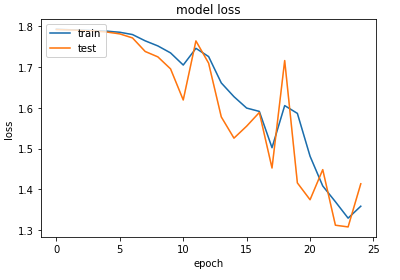
\includegraphics[scale=0.55]{sgd_loss}\\

\section{Wykorzystanie sieci AlexNet}
Sieć o nazwie AlexNet została zaprezentowana przez Alexa Krizhevskyego, Geoffreya Hintona oraz
Ilya Sutskevera w 2012 roku. Jej ideą jest zastosowanie większej ilośći warstw konwolucyjnych,
gdzie początkowe dwie warstwy mają filtry rozmiarów odpowiednio 11x11 oraz 5x5. Następnie
umieszczone są trzy warstwy konwolucyjne z filtrami 3x3, które w przeciwieństwie do pierwszych
dwóch warstw nie są rozdzielone warstwami z maxpoolingiem. AlexNet zdeklasowała rywali
w konkursie ILSVRC 2012 i swoimi rezultatami zszokowała wielu naukowców. Z racji tak świetnych
rekomendacji, zdecydowano się na realizację modelu przypominającego jej budowę.\\
Zastosowanie uproszczonej architektury, bazującej na idei sieci AlexNet pozwoliło
na osiągnięcie poprawności wynoszącej 98.88\% po 25 epokach. Na wykresie uczenia się
można zaobserwować, że przez pierwsze 10 epok prezycja przewidywań sieci w ogólnie nie
rosła. Obserwacja sugeruje, że sieci głębsze mogą potrzebować większej ilości epok
do rozpoczęcia procesu prawidłowego rozpoznawania obrazów.\\
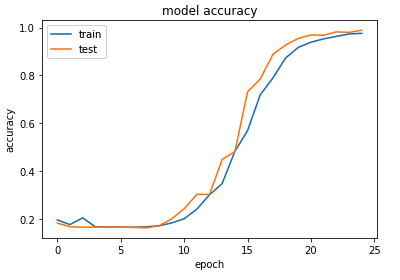
\includegraphics[scale=0.55]{alexnet_acc}
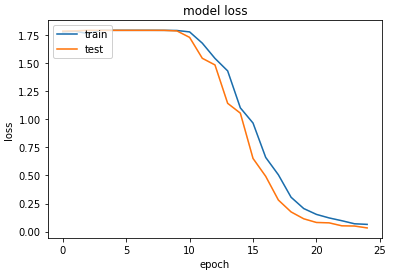
\includegraphics[scale=0.55]{alexnet_loss}

\section{Porównianie dla obrazów kolorowych i czarno-białych}
Obraz w skali szarości posiada jedynie jeden kanał odpowiadający jasności. Obrazy kolorowe RGB
posiadają trzy kanały informujące o nasyceniu odpowiednio czerwonego, zielonego i niebieskiego koloru.
Wzrost ilości informacji wiąże się z większym obciążeniem pamięci i większą ilością parametrów.
W celu weryfikacji różnicy między uczeniem obu rodzajów obrazów podjęto próbę porównania wyników
uczenia dla dwóch jednakowych sieci.\\
\textbf{Kolorowe RGB:}\\
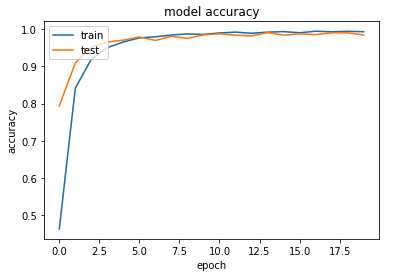
\includegraphics[scale=0.55]{comp_color_acc}
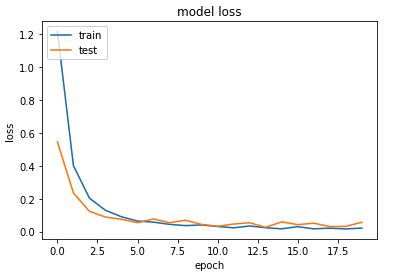
\includegraphics[scale=0.55]{comp_color_loss}\\
\textbf{Skala szarości:}\\
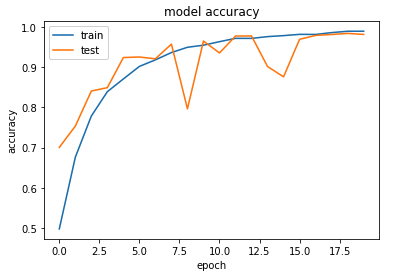
\includegraphics[scale=0.55]{comp_gray_acc}
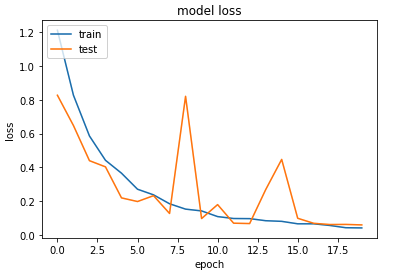
\includegraphics[scale=0.55]{comp_gray_loss}\\
Do tego eksperymentu wykorzystano narzędzie generatora dostępne w Keras, które umożliwia
przekazywanie obrazów do sieci bez konieczności wcześniejszego ładowania całego zbioru
do pamięci, umożliwiając pracę na bardzo dużych zestawach danych. Architektura obu
sieci była uproszczona, by zniwelować długi czas uczenia. Modele obu sieci znajdują się poniżej:\\\\
Oba modele po 20 epokach wykazały się bardzo zbliżonymi wynikami 98,47\% oraz 98,12\%
na korzyść sieci z kolorowymi obrazami. Lepiej radzący sobie model, dodatkowo nauczył
się bardzo szybko do poziomu 95\%, osiągając go już po 4 epoce, gdzie operujący na
obrazach w skali szarości osiągnął ten wynik po 10 epokach. Obserwacja ta może sugerować,
że większa różnica w wartościach dla kolorowych obrazów może przyśpieszać uczenie, ale
wymaga większej ilości pamięći i spowalnia każdą epokę o 15\%.

\section{Porównanie modelu sekwencyjnego i funkcyjnego biblioteki Keras}
\paragraph{Pierwsze użycie modelu funkcyjnego} \mbox{}\\
Standardowym sposobem na stworzenie sieci neuronowej w bibliotece Keras jest wykorzystanie
sekwencyjnego modelu, opierającego się na zasadzie umieszczania warstw na stosie. Bardziej
zaawansowaną możliwością jest wybranie modelu funkcyjnego API, który pozwala na budowę złożonych
sieci neuronowy m.in. z wieloma wyjściami, współdzielonymi warstwami i acyklicznymi grafami.\\
Zdecydowanie większe możliwości modelu funkcyjnego spowodowały chęć realizacji bardziej złożonych
sieci neuronowych. Pierwsza próba miała za zadanie odtworzyć sieć o identycznej budowie jak w
pierwszy model operujący na różnokolorowych zbiorach i porównać wyniki po uczeniu przez 25 epok.
Model został przedstawiony poniżej:\\
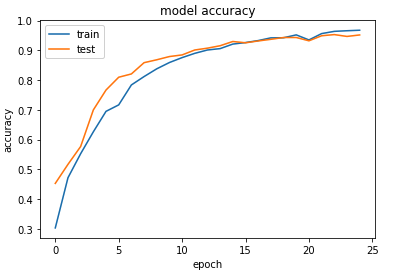
\includegraphics[scale=0.55]{adam_API_acc}
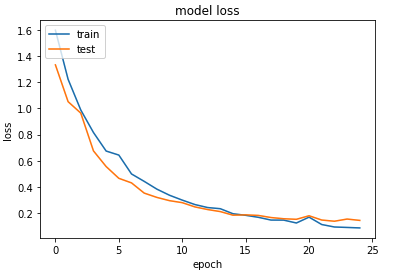
\includegraphics[scale=0.55]{adam_API_loss}\\
Zaskoczeniem była spora rozbieżność w ilości parametrów do nauczenia.W modelu sekwencyjnym
ich ilość wynosiła 18 milionów, a w modelu funkcyjnym API aż 25 milionów parametrów, co oznacza
40\% wzrost ich ilości oraz 50\% wzrost czasu potrzebnego na jedną epokę przy identycznie
zdefiniowanych warstwach. Ciężko uzasadnić tą różnicę, z grafu można wywnioskować, że
prawdopodobnie model ten inaczej uwzględniał filtry konwolucyjne, ponieważ rozmiar warstw
po ich zastosowaniu nie był jednakowy.\\
Niezależnie od tego, model osiagnął zdumiewająco dobry rezultat 95,17\% dokładności.
Wadą tego rozwiązania była, przez zwiększoną ilość parametrów i konieczność zastosowania
mniejszego rozmiaru partii obrazów jednocześnie dostarczanych sieci z powodów
problemów z pamięcią.

\paragraph{Pełne porównanie modeli} \mbox{}\\
Brak sugestii dostępnych w internecie oraz dokumentacji biblioteki Keras wyjaśniających różnice
w ilośc parametrów w modelach sekwencyjnym oraz API spowodował chęć stworzenia dwóch dużych,
identycznych modeli, bezpośrednio porównających ilość parametrów. Modele zostały jedynie
skompilowane w celu wyciągnięcia informacji o ich rozmiarach, ich uczenie zajęło by zbyt dużo czasu.\\
Po kompilacji, model sekwencyjny uzyskał 47 milionów parametrów, a model funkcyjny API
aż 500 milionów parametrów do nauczenia. Ta ogromna różnica spowodowała zaniechanie
kolejnych prac nad modelami funkcyjnymi z uwagi na wielokrotne zwiększenie czasu potrzebnego
na proces uczenia.

\section{Próby wykorzystania prostokątnych obrazów}
\paragraph{Doświadczenia zakończone niepowodzeniem} \mbox{}\\
Dotychczasowe modele korzystały ze zbiorów o obrazach w kształcie kwadratów z kośćmi
umieszczonymi w ich środkowej części. Drugi rodzaj przygotowanych zbiorów danych zwiększał
trudność zadania, dzięki zastosowaniu obrazów prostokątnych z mniejszym obszarem na
którym znajdowała się kostka w stosunku do pierwsze rodzaju obrazów.\\
Po uzyskaniu wielu bardzo dobrych wyników powyżej 90\% na obrazach o rozmiarach 64x64
przystapiono do prób znacznego zwiększenia obrazów prostokątnych.\\
Pierwszą próbą było wykorzystanie obrazów 320x240 zarówno w wersjach kolorowych jak
i w skali szarości. Jeden z modeli bazował na architekturze AlexNet, drugi bezpośrednio
ją kopiował, ale pomimo świetnego wyniku na mniejszych obrazach, w obu przypadkach
uczenie zakończyło się całkowitą klęską. Warto wspomnieć, że czas potrzebny na
jedną epokę był około 15-krotnie większy niż w przypadku obrazów 64x64.\\
Ostania próba z obrazami w tym rozmiarze, zakładała użycie uproszczonej architektury
podobnie jak przy porównaniu uczenia obrazów RGB i w skali szarości. Finalnie, tak jak
wcześniej, pomimo 20 epok sieć nie wykazała żadnego postępu w rozpoznawaniu kości.\\\\
Niepowodzenia spowodowały konieczność zmniejszenia zbiorów przez ograniczenie rozmiarów obrazów.
Problemem podczas zmniejszania była chęć uniknięcia problemów z brakiem ostrości
oczek na kostce co mogłoby uniemożliwić skuteczną naukę. Zdecydowano się na dwukrotne
zmniejszenie rozmiarów obrazów, licząc że pozwoli to na zaobserwowanie chociaż niewielkich
postępów.\\
Sieć bazująca na zdjęciach 160x120 była pierwszą próbą, gdzie zamiast jak dotychczas
kwadratowych, użyto prostokątnych filtrów konwolucyjnych. Proces uczenia po 20 epokach
niestety również zakończył się niepowodzeniem.\\
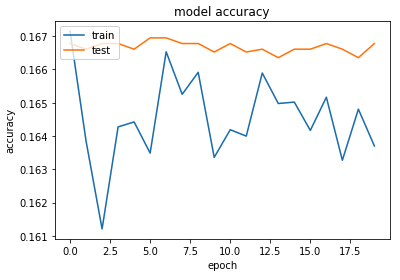
\includegraphics[scale=0.55]{not_learned_acc}
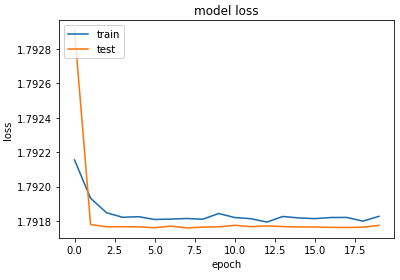
\includegraphics[scale=0.55]{not_learned_loss}

\paragraph{Wytrenowany prostokątny model} \mbox{}\\
Powyższe porażki oraz wcześniejsze sukcesy na kwadratowych obrazach sugerowały, że
prawdopodobnie modele nie są błedne, jedynie obrazy mogą mieć za duży rozmiar. Ta hipoteza
rozpoczeła proces dobierania odpowiedniej rozdzielczości zdjęć tak by były małe, jednocześnie
unikając rozmycia oczek na kostce nie. Najlepszym wyborem okazały się zdjęcia w rozmiarze 106x79,
zachowujące proporcje jak obrazy 160x120, ale posiadające o 50\% mniejszą liczbę parametrów.\\
Pierwsza próba przeprowadzona przez 20 epok z filtrami konwolucjnymi o prostokątnych
kształtach wreszcie zakończyła się sukcesem. Sieć osiągnęła wynik 68,03\% co nie
było świetnym rezultatem, ale dawało informację, że dalsza nauka jest możliwa.\\
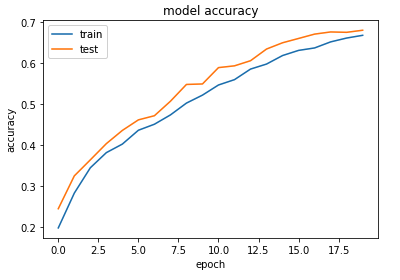
\includegraphics[scale=0.55]{rect_acc}
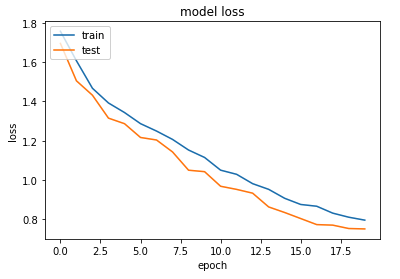
\includegraphics[scale=0.55]{rect_loss}

\section{Doskonalenie modelu z prostokątnymi obrazami}
Po pierwszym sukcesie sieci z obrazami prostokatnymi, podjęto decyzję o jej ulepszeniu.
Zaczęto od próby zmniejszenia ilości parametrów przez zamianę większych filtrów konwolucyjnych,
większą ilością mniejszych, co znacząco zmniejszało ilość parametrów sieci potrzebną do nauczenia
\textit{Substituting Big convolution} \cite{substBigConv}.
Po zaaplikowaniu ulepszeń i nauce sieci, okazało się że sieć nie poprawiła się w żadnym
stopniu. Prawodopodobnym powodem była zmiana architektury sieci wraz z powtórnym
zastosowaniem kwadratowych filtrów.\\
Drugim pomysłem na ulepszenie sieci było zastosowanie zastępowania większych filtrów
kilkoma mniejszymi połączonego ze zamianą funkcji aktywacji ReLU na LeakyReLU w celu uniknięcia
możliwych do wystąpienia problemów z zanikającym neuronem. Ulepszenie jednak podobnie
jak wcześniejsze nie sprawdziło się w ogóle i nie umożliwiło poprawy dokładności sieci.

\section{Najskuteczniejszy model z prostokątnymi obrazami}
Wykres procesu uczenia sieci z obrazami 106x79 kształtem przypominał funkcję logarytmiczną
co nasuneło pomysł ze zwiększeniem ilości epok. Podjęto decyzję o kontynuacji uczenia
do kolejno 40, 60, 80 i 100 epok.\\
Podejście to okazało się bardzo skuteczne, ponieważ po każdych 20 epokach
sieć odnosiła lepsze rezultaty, które prezentowały się nastepująco:\\
20 epok: 68,03\%\\
40 epok: 78,21\%\\
60 epok: 81,59\%\\
80 epok: 82,39\%\\
100 epok: 84,67\%\\
\begin{sidewaysfigure}
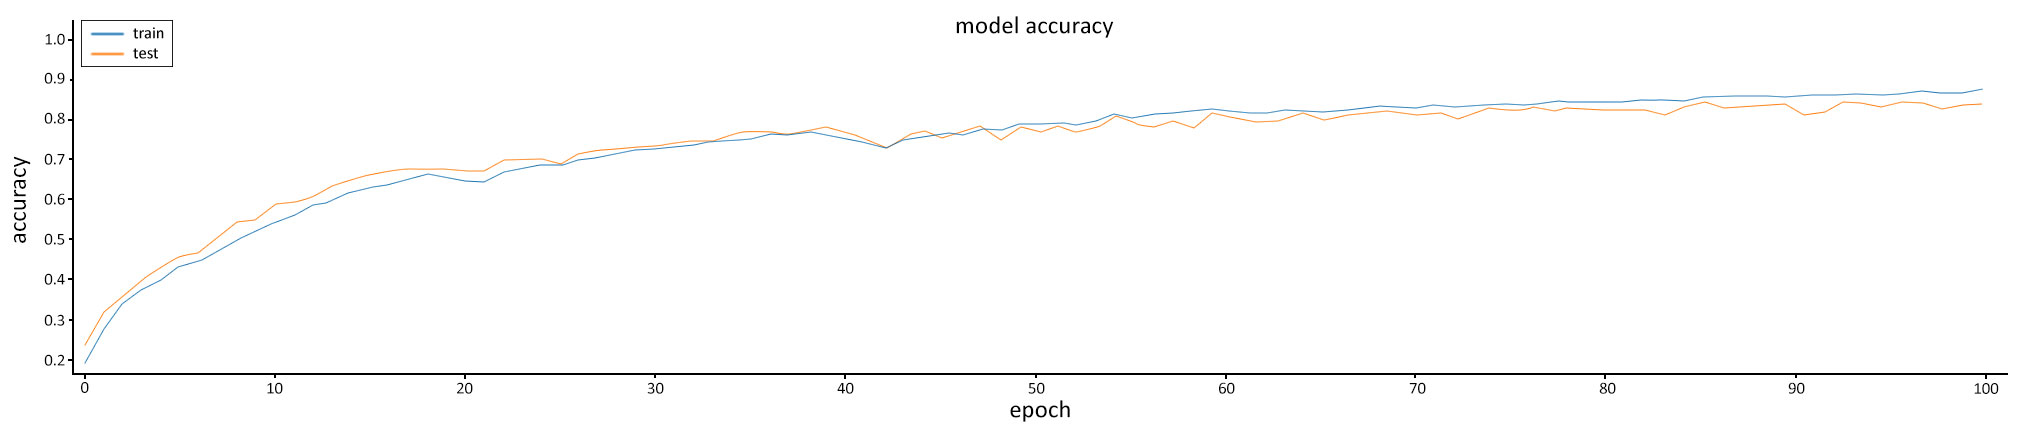
\includegraphics[scale=0.36]{wykres_100}
\caption{Wykres uczenia przez 100 epok}
\end{sidewaysfigure}
Wyniki uświadamiają, że prawdopodobnie nawet nieudane próby z większymi zdjęciami
mogłyby się powieść, konieczne byłoby jedynie zwiększenie ilości epok. Wiąże się to jednak
z ogromnym nakładem czasu, ponieważ prawdopodobnie sensowne rezultaty można by osiągnąć
dopiero po 100 epokach.


% !TEX encoding = UTF-8 Unicode

\chapter{Podsumowanie}

Zwieńczeniem całej pracy i stworzonych modeli są dwa skrypty rozpoznające ilość
oczek wyrzuconych na kości w czasie rzeczywistym. Programy korzystają z wytrenowanych
modeli załadowanych do pamięci, które analizują obraz dostarczany z kamery
podłączonej do komputera. Modele są przystosowane do rozpoznawania kości na
obrazach o wielkościach 64x64 oraz 106x79 pikseli.\\
Obraz dostarczany z kamery jest wielokrotnie większy, co wymusiło wyznaczenie jego
części, która jest analizowana przez zaaplikowane sieci neuronowe. Ta część obrazu
oznaczona jest białymi krawędziami dla łatwiejszego zlokalizowania miejsca, w którym
powinna być umieszczona kość pod kamerą.
Dla obrazów 64x64 wykonano kilka modeli sieci, które osiągnęły powyżej 90\% skuteczności.
Program umożliwia porównanie wyników dzięki zaaplikowaniu ich do analizy tego
samego obszaru na zdjęciu. Pozwala to zauważyć między innymi lepsze rozpoznawanie
pewnych kombinacji kolorystycznych niektórych modeli lub trudności z rozróżnieniem
wyrzuconych czterech oczek od sześciu, z uwagi na efekt zlewania się ich podczas
skalowania.\\
Dla obrazów 106x79 zaaplikowany jest jedynie jeden model, wytrenowany przez 100 epok.\\
Wyniki zaobserwowane podczas prac związanych z tworzeniem sieci neuronowych przyniosły
wiele niespodziewanych sytuacji. Często otrzymywane wyniki były zdumiewające,
biorąc pod uwagę, jak drobne różnice w budowie sieci wpływały na końcowe rezultaty.
Największym zaskoczeniem były bardzo duże problemy z uczeniem obrazów prostokątnych w
porównaniu do obrazów kwadratowych. Za przykład może posłużyć mniejsza o jedną trzecią
ilości danych w obrazach w skali szarości i rozmiarze 106x79 pikseli w stostunku do
obrazów kolorowych i rozmiaru 64x64 piksele. Proces uczenia się przebiegał trzykrotnie
dłużej na jedną epokę i zastosowanie pięciokrotnie większą ilości epok. Mimo to, wynik
dla obrazów kwadratowych wyniósł 98,47\%, a dla prostokątnych 84,67\%.\\
Wszystkie eksperymenty pokazały, że nawet proste zadanie rozpoznawania oczek na kostce
wymaga dużej ilości danych i mocy obliczeniowej, by w uzyskać satysfakcjonujące wyniki.
Przykład ten pokazuje także jak wiele zastosowań może mieć zyskujące na popularności
uczenie maszynowe, które wraz z rozwojem technologii będzie mieć coraz więcej możliwości
na dostosowywania algorytmów do określonych danych.


% !TEX encoding = UTF-8 Unicode
\addcontentsline{toc}{chapter}{Bibliografia}
\begin{thebibliography}{99}

\bibitem{CS231n}
Stanford University course CS231n
\\\texttt{http://cs231n.github.io/convolutional-networks/}

\bibitem{CS231n_backprop}
Stanford University course CS231n
\\\texttt{http://cs231n.github.io/optimization-2/}

\bibitem{CS231n_activ}
Stanford University course CS231n
\\\texttt{http://cs231n.github.io/neural-networks-1/}

\bibitem{NNbiology}
Eric Roberts, Stanford University
\\\texttt{https://cs.stanford.edu/people/eroberts/courses/soco/projects/\\neural-networks/}

\bibitem{NeuronAnimation}
Tuples Edu
\\\texttt{https://becominghuman.ai/what-is-an-artificial-neuron-8b2e421ce42e}

\bibitem{needForBias}
Jaron Collis
\\\texttt{https://medium.com/deeper-learning/glossary-of-deep-learning-bias\\-cf49d9c895e2}

\bibitem{substBigConv}
Leonardo Araujo dos Santos
\\\texttt{https://leonardoaraujosantos.gitbooks.io/artificial-inteligence/\\content/convolutional\_neural\_networks.html}

\bibitem{backprop}
Leonardo Araujo dos Santos
\\\texttt{https://leonardoaraujosantos.gitbooks.io/artificial-inteligence/\\content/backpropagation.html}

\bibitem{typesOfOptimizationAlgorithms}
Anish Singh Walia
\\\texttt{https://towardsdatascience.com/types-of-optimization-algorithms-\\used-in-neural-networks-and-ways-to-optimize-gradient-95ae5d39529f}

\bibitem{intuitiveExplanation}
Ujjesl Karn
\\\texttt{https://ujjwalkarn.me/2016/08/11/intuitive-explanation-convnets/}

\bibitem{NNArchitectures}
Eugenio Culurciello
\\\texttt{https://towardsdatascience.com/neural-network-architectures-156e\\5bad51ba}

\bibitem{activationFunctions}
Avinash Sharma V
\\\texttt{https://medium.com/the-theory-of-everything/understanding-activa\\tion-functions-in-neural-networks-9491262884e0}

\bibitem{activationFunctionsV2}
Sagar Sharma
\\\texttt{https://towardsdatascience.com/activation-functions-neural-netwo\\rks-1cbd9f8d91d6}

\bibitem{XORproblem}
Aditya V. D
\\\texttt{https://becominghuman.ai/neural-network-xor-application-and-fund\\amentals-6b1d539941ed}

\bibitem{WIKIfeedforward}
\\\texttt{https://en.wikipedia.org/wiki/Feedforward\_neural\_network}

\bibitem{WIKIcnn}
\\\texttt{https://en.wikipedia.org/wiki/Convolutional\_neural\_network}

\bibitem{WIKIrectifier}
\\\texttt{https://en.wikipedia.org/wiki/Rectifier\_(neural\_networks)}

\bibitem{WIKIimageRecognition}
\\\texttt{https://en.wikipedia.org/wiki/Computer\_vision\#Recognition}

\bibitem{MNIST}
Yann LeCun, Corinna Cortes, Christoper J.C. Burges
\\\texttt{http://yann.lecun.com/exdb/mnist/}

\bibitem{CIFAR-10}
Alex Krizhevsky
\\\texttt{https://www.cs.toronto.edu/\char`\~kriz/cifar.html}

\bibitem{AlexNetdesc}
Adit Deshpande
\\\texttt{https://adeshpande3.github.io/The-9-Deep-Learning-Papers-You-Need\\-To-Know-About.html}

\bibitem{AlexNetNVIDIA}
Alex Krizhevsky, Ilya Sutskever, Geoffrey E. Hinton
\\\texttt{https://www.nvidia.cn/content/tesla/pdf/machine-learning/imagenet-\\classification-with-deep-convolutional-nn.pdf}

\bibitem{AlexNetpresentation}
Tugce Tasci, Kyunghee Kim
\\\texttt{http://vision.stanford.edu/teaching/cs231b\_spring1415/slides/alex\\net\_tugce\_kyunghee.pdf}

\bibitem{DropConnect}
Li Wan, Matthew Zeiler, Sixin Zhang, Yann LeCun, Rob Fergus
\\\texttt{https://cs.nyu.edu/\char`\~wanli/dropc/}

\bibitem{DropoutPreventOverfit}
Jason Morrison
\\\texttt{https://medium.com/paper-club/paper-review-dropout-a-simple-way-\\to-prevent-neural-networks-from-overfitting-4f25e8f2283a}

\bibitem{understandingConv}
Matthew D. Zeiler, Rob Fergus
\\\texttt{https://arxiv.org/abs/1311.2901}

\bibitem{OptimizersOverview}
Sebatian Ruder
\\\texttt{http://ruder.io/optimizing-gradient-descent/}

\bibitem{AdamOptimizer}
Diederik P.Kingma, Jimmy Ba
\\\texttt{https://arxiv.org/abs/1412.6980}

\bibitem{konwolucja}
Krzysztof Sopyła
\\\texttt{https://ksopyla.com/python/operacja-splotu-przetwarzanie-obrazow/}

\bibitem{whyNotMSE}
James D. McCaffrey
\\\texttt{https://jamesmccaffrey.wordpress.com/2013/11/05/why-you-should-use\\-cross-entropy-error-instead-of-classification-error-or-mean-squared-\\error-for-neural-network-classifier-training/}

\end{thebibliography}


% !TEX encoding = UTF-8 Unicode

\chapter{Dodatek A - zbiory danych}
Zbiory danych wykorzystane do uczenia przedstawionych modeli sieci neuronowych
znajdują się w linkach dostępnych poniżej:

\paragraph{Zbiór 64x64x1, obrazy w skali szarości, opisany w częsci 5.1} \mbox{}\\
\texttt{https://drive.google.com/open?id=1-qCVGTql6A3QHLxS0aQvhFxSz5wUY7uG}

\paragraph{Zbiór 64x64x3, obrazy kolorowe, opisany w częsci 5.1} \mbox{}\\
\texttt{https://drive.google.com/open?id=1oWa8t5pCWCGyC3Mbdn_XJ2hVdf0yqrMu}

\paragraph{Zbiór 106x79x1, obrazy w skali szarości, opisany w części 5.2} \mbox{}\\
\texttt{https://drive.google.com/open?id=1JS_C_pJqU2TmBEVvMTULTXue7VZJKONH}


% !TEX encoding = UTF-8 Unicode

\chapter{Dodatek B - modele sieci neuronowych} \label{dodatekB}

Wszystkie modele sieci neuronowych przedstawione w pracy dostępne są pod linkami
podanymi poniżej:
\section{Obrazy kwadratowe 64x64}
\paragraph{Pierwszy model z obrazami w jednej kolorystyce} \mbox{}\\
\texttt{https://github.com/oziomek1/NNLearning/blob/master/dices\_cnn/dice\_cnn.ipynb}

\paragraph{Pierwszy model ze zróżnicowanymi zdjęciami} \mbox{}\\
\texttt{https://github.com/oziomek1/neural\_network\_dice/blob/master/dice\_cnn\_adam.ipynb}

\paragraph{Model z wybranymi zdjęciami} \mbox{}\\
\texttt{https://github.com/oziomek1/neural\_network\_dice/blob/master/dice\_cnn\_adam\\\_wybrane.ipynb}

\paragraph{Modele do analizy optymalizatorów} \mbox{}\\
Optymalizator Adam:\\
\texttt{https://github.com/oziomek1/neural\_network\_dice/blob/master/dice\_cnn\_adam.ipynb}
Optymalizator RMSprop:\\
\texttt{https://github.com/oziomek1/neural\_network\_dice/blob/master/dice\_cnn\\\_rmsprop.ipynb}
OptymalizatorSGD:\\
\texttt{https://github.com/oziomek1/neural\_network\_dice/blob/master/dice\_cnn\_sgd.ipynb}

\paragraph{Model oparty o AlexNet} \mbox{}\\
\texttt{https://github.com/oziomek1/neural\_network\_dice/blob/master/generator\\\_AlexNet.ipynb}

\paragraph{Porównanie modeli dla obrazów kolorowych i w skali szarości} \mbox{}\\
Obrazy kolorowe:\\
\texttt{https://github.com/oziomek1/neural\_network\_dice/blob/master/generator\\\_comparison.ipynb}
\\Obrazy w skali szarości:\\
\texttt{https://github.com/oziomek1/neural\_network\_dice/blob/master/generator\\\_comparison\_gray.ipynb}

\paragraph{Pierwszy model funkcyjny} \mbox{}\\
\texttt{https://github.com/oziomek1/neural\_network\_dice/blob/master/dice\_cnn\_API.ipynb}

\paragraph{Pełne porównanie modelu funkcyjnego i sekwencyjnego} \mbox{}\\
\texttt{https://github.com/oziomek1/neural\_network\_dice/blob/master/API\_Sequential\\\_®Keras2.ipynb}

\section{Obrazy prostokątne}
\paragraph{Trzy nienauczone modele z prostokątnymi obrazami 320x240} \mbox{}\\
\texttt{https://github.com/oziomek1/neural\_network\_dice/blob/master/generator\_320x\\240\_AlexNet.ipynb}\\
\texttt{https://github.com/oziomek1/neural\_network\_dice/blob/master/generator2\_320x\\240\_AlexNet.ipynb}\\
\texttt{https://github.com/oziomek1/neural\_network\_dice/blob/master/generator3\_320x\\240.ipynb}

\paragraph{Model ze protokątnymi obrazami 160x120} \mbox{}\\
\texttt{https://github.com/oziomek1/neural\_network\_dice/blob/master/simple\_NN\\\_160x120.ipynb}

\paragraph{Nauczony model z prostokątnymi obrazami 106x79} \mbox{}\\
\texttt{https://github.com/oziomek1/neural\_network\_dice/blob/master/simple\_NN\\\_106x79.ipynb}

\paragraph{Ulepszanie modelu przez redukcje dużych konwolucji} \mbox{}\\
\texttt{https://github.com/oziomek1/neural\_network\_dice/blob/master/substituting\\\_106x79.ipynb}

\paragraph{Ulepszanie modelu przez LeakyReLU} \mbox{}\\
\texttt{https://github.com/oziomek1/neural\_network\_dice/blob/master/subst\_LReLU\\\_106x79.ipynb}

\paragraph{Kontynuacja uczenia jedynego nauczonego modelu 20-60 epok} \mbox{}\\
\texttt{https://github.com/oziomek1/neural\_network\_dice/blob/master/simple\_NN\\\_106x79\_continue.ipynb}

\paragraph{Kontynuacja uczenia jedynego nauczonego modelu 60-100 epok} \mbox{}\\
\texttt{https://github.com/oziomek1/neural\_network\_dice/blob/master/simple\_NN\\\_106x79\_continue\_80\_100.ipynb}


\end{document}
